%%
%% This is file `sample-acmsmall-biblatex.tex',
%% generated with the docstrip utility.
%%
%% The original source files were:
%%
%% samples.dtx  (with options: `acmsmall-biblatex')
%% 
%% IMPORTANT NOTICE:
%% 
%% For the copyright see the source file.
%% 
%% Any modified versions of this file must be renamed
%% with new filenames distinct from sample-acmsmall-biblatex.tex.
%% 
%% For distribution of the original source see the terms
%% for copying and modification in the file samples.dtx.
%% 
%% This generated file may be distributed as long as the
%% original source files, as listed above, are part of the
%% same distribution. (The sources need not necessarily be
%% in the same archive or directory.)
%%
%%
%% Commands for TeXCount
%TC:macro \cite [option:text,text]
%TC:macro \citep [option:text,text]
%TC:macro \citet [option:text,text]
%TC:envir table 0 1
%TC:envir table* 0 1
%TC:envir tabular [ignore] word
%TC:envir displaymath 0 word
%TC:envir math 0 word
%TC:envir comment 0 0
%%
%%
%% The first command in your LaTeX source must be the \documentclass command.
\documentclass[sigconf,natbib=false]{acmart}

%%
%% \BibTeX command to typeset BibTeX logo in the docs
\AtBeginDocument{%
  \providecommand\BibTeX{{%
    Bib\TeX}}}

%% Rights management information.  This information is sent to you
%% when you complete the rights form.  These commands have SAMPLE
%% values in them; it is your responsibility as an author to replace
%% the commands and values with those provided to you when you
%% complete the rights form.
\setcopyright{acmcopyright}
\copyrightyear{2018}
\acmYear{2018}
\acmDOI{XXXXXXX.XXXXXXX}


%%
%% Submission ID.
%% Use this when submitting an article to a sponsored event. You'll
%% receive a unique submission ID from the organizers
%% of the event, and this ID should be used as the parameter to this command.
%%\acmSubmissionID{123-A56-BU3}

%%
%% For managing citations, it is recommended to use bibliography
%% files in BibTeX format.
%%
%% You can then either use BibTeX with the ACM-Reference-Format style,
%% or BibLaTeX with the acmnumeric or acmauthoryear sytles, that include
%% support for advanced citation of software artefact from the
%% biblatex-software package, also separately available on CTAN.
%%
%% Look at the sample-*-biblatex.tex files for templates showcasing
%% the biblatex styles.
%%


%%
%% The majority of ACM publications use numbered citations and
%% references, obtained by selecting the acmnumeric BibLaTeX style.
%% The acmauthoryear BibLaTeX style switches to the "author year" style.
%%
%% If you are preparing content for an event
%% sponsored by ACM SIGGRAPH, you must use the acmauthoryear style of
%% citations and references.
%%
%% Bibliography style
\RequirePackage[
  datamodel=acmdatamodel,
  ]{biblatex}

\usepackage{xspace}
\usepackage{float}
\newcommand{\greedy}{\textsc{Greedy Selection}\xspace}
\newcommand{\jogging}{\textsc{Jogging Tour}\xspace}
\newcommand{\ils}{\textsc{Iterative Local Search}\xspace}
\newcommand{\ilp}{\textsc{Integer Linear Programming}\xspace}
\newcommand{\AOP}{\textsc{AOP}\xspace}
\newcommand{\III}{\mathcal{I}}

%% Declare bibliography sources (one \addbibresource command per source)
\addbibresource{references.bib}

%%
%% end of the preamble, start of the body of the document source.
\begin{document}

%%
%% The "title" command has an optional parameter,
%% allowing the author to define a "short title" to be used in page headers.
\title{Tour4Me: A Framework for Customized Tour Planning Algorithms}

%%
%% The "author" command and its associated commands are used to define
%% the authors and their affiliations.
%% Of note is the shared affiliation of the first two authors, and the
%% "authornote" and "authornotemark" commands
%% used to denote shared contribution to the research.

\author{Kevin Buchin}
\orcid{1234-5678-9012}
\affiliation{%
  \institution{TU Dortmund}
  \city{Dortmund}
  \country{Germany}
}
\email{kevin.buchin@tu-dortmund.de}

\author{Mart Hagedoorn}
\orcid{1234-5678-9012}
\affiliation{%
  \institution{TU Dortmund}
  \city{Dortmund}
  \country{Germany}
}
\email{mart.hagedoorn@tu-dortmund.de}

\author{Guangping Li}
\orcid{1234-5678-9012}
\affiliation{%
  \institution{TU Dortmund}
  \city{Dortmund}
  \country{Germany}
}
\email{guangping.li@tu-dortmund.de}

%%
%% By default, the full list of authors will be used in the page
%% headers. Often, this list is too long, and will overlap
%% other information printed in the page headers. This command allows
%% the author to define a more concise list
%% of authors' names for this purpose.
\renewcommand{\shortauthors}{Buchin, Hagedoorn, and Li}
\newcommand{\tM}{\textsc{Tour4Me}\xspace}

%%
%% The abstract is a short summary of the work to be presented in the
%% article.
\begin{abstract}
The touring problem aims to find an ``interesting'' (round) trip of a given length. Here, what is considered interesting depends on the type of the desired route, e.g., an user may be looking for a off-road cycling trip or fast running route.
There are two main perspectives on the touring problem, maximizing profit or minimizing cost, which result in very different algorithmic solutions. We provide a framework that allows for straightforward integration of new algorithms for both perspectives on the touring problem.
In this demonstration we have included a new exact solver, a heuristic, and two greedy methods. The user can experiment with the algorithms and different profits/costs. The generated tours can be explored in an easy-to-use web interface.
\end{abstract}

%%
%% The code below is generated by the tool at http://dl.acm.org/ccs.cfm.
%% Please copy and paste the code instead of the example below.
%%
\begin{CCSXML}
<ccs2012>
   <concept>
       <concept_id>10003033.10003068.10003073.10003077</concept_id>
       <concept_desc>Networks~Network design and planning algorithms</concept_desc>
       <concept_significance>500</concept_significance>
       </concept>
   <concept>
       <concept_id>10002951.10003227.10003236.10003237</concept_id>
       <concept_desc>Information systems~Geographic information systems</concept_desc>
       <concept_significance>300</concept_significance>
       </concept>
   <concept>
       <concept_id>10003752.10003809.10003636.10003811</concept_id>
       <concept_desc>Theory of computation~Routing and network design problems</concept_desc>
       <concept_significance>300</concept_significance>
       </concept>
 </ccs2012>
\end{CCSXML}

\ccsdesc[500]{Networks~Network design and planning algorithms}
\ccsdesc[300]{Information systems~Geographic information systems}
\ccsdesc[300]{Theory of computation~Routing and network design problems}
%%
%% Keywords. The author(s) should pick words that accurately describe
%% the work being presented. Separate the keywords with commas.
\keywords{Touring problem, Trip routing, Arc orienteering}

\thanks{Source code and web interface of Tour4Me at \url{https://tramectory.github.io/tour4me/}.}

%%
%% This command processes the author and affiliation and title
%% information and builds the first part of the formatted document.
\maketitle

\section{Introduction}

% Problem description and motivation
Most people who do outdoor activities run into the problem of finding an appropriate route. 
Depending on the activity from hiking and jogging to gravel and road cycling, requirements from individual users can greatly vary.
To this end we developed the framework \tM for computing customized round trips. 
The tool \tM includes four touring algorithms and provides an intuitive web interface to create tours following users specific demands and preferences. 

In this work, we introduce the touring problem, which is defined formally as follows. 
Let $G$ be an undirected graph consisting of a vertex set $V$ and a set $E$ of edges. Furthermore, we are given a cost function $w{:}\ E \rightarrow \mathbb{N}$ and a profit function $\pi{:}\ E \rightarrow \mathbb{N}$ assigning different cost (distance or time) and profit to each edge of $G$.
We can generalize the terms cost and profit to paths. 
Given a path $P = (e_1, \cdots, e_{\ell})$ of $G$, we denote the cost of $P$ as $w(P)$, which is defined as $\sum_{i=1}^{\ell} w(e_i)$; and for the profit of $P$ we write $\pi(P) = f(P) + \sum_{ e \in \bigcup{e_i \mid 1 \leq i \leq \ell } } \pi(e)$.
Here $f(P)$ can be any additional quality function based on the global structure of the path.
Given a cost budget $B$ and a starting vertex $s$, the objective of touring problem is to find a cycle $P=(e_1, \cdots, e_{\ell})$ starting and ending at the vertex $s$ that maximizes the profit $\pi(P)$ within the cost budget $c(P) \leq B$. 
Note that in the touring problem it is allowed to visit an edge multiple times, but its profit is only counted once.

In this work we consider the area covered by $P$ as our additional quality measure $f(P)$. The idea is that an user can prefer a route resembling a circle over a long thin strip or a route with lots of intersections. The higher the covered area the closer a route resembles this circle. 
We use the shoelace method for calculating the area \cite{meister1769generalia}. 
Not only can we efficiently calculate the area after modifying sections of a route, but this method will also force the tour to from a simple polygon with nodes in a clockwise order.
Having a clockwise tour is additionally beneficial as this results in more right turns than left turns, which in most countries means less crossings of streets and having more traffic priority.
Furthermore, in \tM, developers can easily add additional measures and users can choose what they find important for their own route.

There exist two perspectives for solving the touring problem. The first is the perspective of maximizing profit as with the \emph{arc orienteering problem} (AOP). The arc orienteering is closely related to the well-studied \emph{orienteering problem} (OP), both of which are NP-hard \cite{chekuri2012improved, bansal2004approximation, blum2007approximation}.
In the OP, given an (un)directed graph, a cost function on edges and a profit function for nodes, the goal is to find a path which maximizes the total collected profit while not violating the budget constraint.
Motivated by creating scenic routes the AOP gives a profit function on arcs or edges instead of nodes to better represent desirable roads.
Verbeeck et al. \cite{verbeeck2014extension} propose a branch-and-cut algorithm that can solve the AOP exactly and a iterative local search metaheuristic for solving larger instance.
Lu et al. \cite{lu2015arc} followed up by introducing spatial database techniques to improve the iterative local search from Verbeeck et al.
Furtermore, the touring problem is a variant of the AOP, when $f(P) = 0$ the touring problem becomes the AOP with fixed start- and endpoints.


The second perspective is perhaps more intuitive and involves minimizing cost. 
Here edges that are desirable are reduced in cost resulting in a new graph $G'$ representing the underlying streets. 
The shortest path between two points in $G'$ now prefers roads that were reduced in cost.
In order to create a cyclic tour with the minimizing cost approach, intermediate waypoints need to be chosen. Between these waypoints the shortest paths on the modified graph are stitched together creating a cyclic tour. The goal is to choose these waypoints such that the aforementioned profit is maximized.
This method is somewhat popular and has received some attention \cite{jogging, stroobant2018generating}. These methods firstly focus on finding a route of the desired length and then softly optimizing for profit.

% \subparagraph*{\textbf{Related Work.}}
% In the orienteering problem (OP), given an (un)-directed graph, the goal is to find a path which maximizes the total collected profit while not violating the budget constraint. In the classic model, a cost is assigned to each edge/arcs and a profit is assigned to each vertex. The profit of a path is defined by the sum of collected profit of its visited vertices. 
% The orienteering problem is well-studied since decades and finds applications in the fields . 
% Motivated by cycling routing problem, the variant arc orienteering problem (AOP) was introduced and has been studied in. In this variant, the profit is assigned to each edge and the profit of a path is defined by the sum of collected profits of each visited edge.
% The touring problem is a variant of the  arc orienteering problem where the goal is to find a cycle with a fixed starting point. 


\subparagraph*{\textbf{Contribution.}}
Our contribution is twofold. Firstly, we designed a prototype tool \tM for generating customized round trip. Here the user can give their priorities and preferences of road types and then the selected algorithm will compute a round trip with customized weights and profits; see Section~\ref{sec:system}.
Using the pipeline of \tM, development of new algorithms can be made more accessible. Data loading and visualization is all handled by \tM, leaving only the algorithm development open without overhead. 
Secondly, in this framework, we implemented four algorithms for touring problems; see Section~\ref{sec:algo}.
We selected one simple greedy approach, two representative sophisticated heuristics for AOP problem and one exact solver based on our introduced (integer linear programming) model for the touring problem.



\section{System}
\label{sec:system}

\begin{figure}[b]
    \centering
    \includegraphics{fig/architecture.pdf}
    \caption{System architecture}
    \label{fig:architecture}
\end{figure}

\subparagraph*{\textbf{Architecture.}}
Our framework is a one-page web application. For the implementation of efficient algorithms in back-end, we use C++, the system architecture can be seen in Fig. \ref{fig:architecture}. 
A simple REST API is hosted using \emph{libhttpserver}\footnote{\url{https://github.com/etr/libhttpserver}} that responds to requests for returning the web interface and route calculations. 
Calculations are requested using \texttt{GET} requests and processed by our request handler. 
Here a problem instance is created with the correct underlying data and user preferences. 
Thereafter, we create one of the algorithm instances which inherent the Solver class, this instance is then used to solve the aforementioned problem.
The result given by the algorithm is returned to the web interface and displayed to the user.

\subparagraph*{\textbf{Data.}}
For this demonstration we have stored a sequence of overlapped map tiles representing the street network as separate files on the server.
When an user request the generation of a route, the system calculates which of the graphs suits the starting point best and loads this graph into its system memory.
The overlapping map tiles are downloaded from \emph{OpenStreetMap}\footnote{\url{https://www.openstreetmap.org/}} (OSM) using \emph{OSMnx}, as introduced by \cite{BOEING2017126}. 
OSMnx downloads and topologically simplifies the raw data from OSM in order to reduce the graph size. 
The resulting graphs are stored in a file following a modified version of the DIMACS\footnote{\url{http://lcs.ios.ac.cn/~caisw/Resource/about_DIMACS_graph_format.txt}} naming convention.

Nevertheless, the graphs representing the true road network still have roughly 100.000 nodes, which is too large for exact methods. 
Therefore, we aim to reduce the graph size by selecting a set of ``interesting'' edges and simplifying the induced graph by the selected edges. 
We simplify the induced graph with OSMnx and denote the resulting graph as the \emph{backbone} of the original graph.
The backbone should only represent interesting features of the original street network and have a greatly reduced the size of the graph.
To demonstrate the backbone we have chosen roads that are part of a bicycle routes that are maintained by local and regional governments, as these are handpicked to be suitable for cycling.
In OSM these roads are part of a relation with the \texttt{route} tag set to \texttt{bicycle}.
To download the backbone we have modified OSMnx to not only download segments, but instead only the relations and from there extract these road segment.
Thereafter, we export the result in a similar manner as the full graphs.

\subparagraph*{\textbf{Interface.}}
\begin{figure}
    \centering
    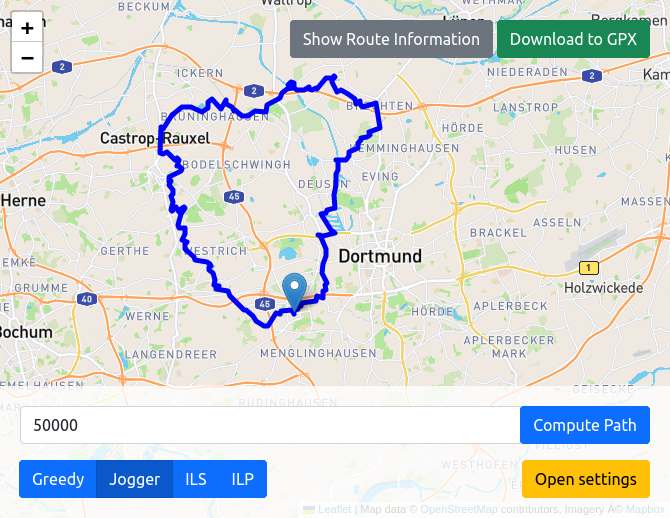
\includegraphics[width=0.45\textwidth]{fig/UIroute.png}
    \caption{The web interface with a calculated route.}
    \label{fig:ui_index}
\end{figure}

\begin{figure}
    \centering
    \includegraphics[width=0.45\textwidth]{fig/UIsettings.png}
    \caption{Settings panel controlling the user's preferences.}
    \label{fig:ui_settings}
\end{figure}

The user interface, shown in Fig. \ref{fig:ui_index}, consists of a large background map. The starting point can be selected by clicking on a spot directly in the map and the target distance can be specified. In order to have more control, an user can open the settings and will be presented with more options as is shown in Fig. \ref{fig:ui_settings}.
The first choice we present is the choice of backbone versus the full data from OSM, using the backbone is faster but could give inferior results.
The next choice consists of a list of road types (\texttt{highway} tag in OSM) and surface types (\texttt{surface} tag).
For each tag the user can choose to leave edges with this tag with zero, positive or negative profit.
Additionally, the user can choose how long the algorithm should run. This setting is more applicable for longer calculations like the algorithms described in Sections \ref{alg:ILS} and \ref{alg:ILP}.
Finally, the user chooses what they find more important, edge profit or covered area, more attributes could be added to this section by developers.

Once the user is satisfied with their decisions they can start computing the path. The server will receive a \texttt{GET} request containing all information about the user preferences. Using these preferences the server will calculate a route with the selected algorithm and respond with a \texttt{JSON}\footnote{\url{https://www.json.org/}} file containing route information. This route will be displayed, as is also shown in Fig. \ref{fig:ui_index}, and route details can be viewed. These details contain metadata like the length and quality of the route. Finally, the route can be exported to a \texttt{GPX}\footnote{\url{www.topografix.com/gpx.asp}} file and loaded on a navigation device such that the route could be used.
%\begin{figure}[htb]
%\centering
%\includegraphics[width=\textwidth]{figs/guis}
%$\caption{The graphical user interface of the developed prototype.}
%\label{fig:GUI}		
%\end{figure}
\section{Algorithm}
\label{sec:algo}
We implemented four representative algorithms in our framework. The simplest approach \greedy is a fast greedy approach which greedily selects edges of high profits.
The second greedy algorithm \jogging aims to obtain a cycle consisting of edges of low costs and high profits.  
Next, we implemented a meta-heuristic \ils. 
This algorithm starts with the greedy solution computed by \greedy and improves the initial solution by applying iterative local search, which also gives the name to our algorithm.
Finally, we propose an integer linear program model for the touring problem. 
To solve our ILP model, we use the MILP solver \emph{GUROBI}\footnote{https://www.gurobi.com/} under the academic license. 
The two more sophisticated algorithms \ils and \ilp also support area maximization. 


%
\subsection{Greedy Selection}
%The greedy selection algorithm uses a straightforward greedy choice for selecting 
%For this iteration we have implemented four dirrent algorithms for calulation and improvement of routes.

The greedy approach \greedy computes a cycle starting at the vertex $s$ by iteratively picking edges of the highest profit. To make sure the computed path is a valid cycle, we only pick edges, from whose endpoint the vertex $s$ can be reached by the remaining cost budget. 
We call such edges valid candidates. 
The algorithm starts by picking an valid edge starting at $s$ of the highest profit. 
Next, we update the remaining cost budget and repeat this greedy selection from the endpoint of the new selected edge until reaching the starting vertex $s$ or reaching a vertex with no valid candidates. 
If the process terminates at a vertex $v$ other than $s$, we add the shorted path from $v$ to $s$ in order to complete the solution. 

\subsection{Jogging Tour}\label{alg:jogging}
We further selected one representative existing approach \jogging~\cite{jogging} for the \AOP problem.
In contract to \greedy approach, this approach takes the edge costs into account and tries to select the ``efficient'' edges, that are edges of high profit and low cost. 
For this, we introduce the metric \textsc{Inefficiency} \xspace on the edges $\gamma: E-> R_{+}$. For each edge $e \in E$, we set $\gamma(e) = \frac{w(e)}{\pi(e) + 0.1}$.
Intuitively, this approach aims to obtain an equilateral triangles consisting of three efficient paths, each of which has a cost close to  $\frac{B}{3}$, and having $s$ as one of the triangle's edge. Firstly, we run a shortest path computation (with Dijkstra’s algorithm) from $s$
using this metric inefficiency.
For each vertex $u,v$, we refer to $P_{u,v}$ as the shortest path of the metric inefficiency in the following.   
We now determine the vertices whose shortest path from $s$ has cost in the range $[\frac{B}{3}- \frac{B}{10} , \frac{B}{3} + \frac{B}{10}]$. We refer to the set of such candidate vertices as the \textit{ring} of $s$ $R_s$.
Next, for each candidate vertex $v$ of $s$, we run a shortest path computation from $v$ and compute the ring $R_v$. Now, we consider the intersection $I_{s,v}$ of two ring sets $R_s$ and $R_v$. Note that the distances from each vertex $u\in I_{s,v}$ to $s$ and $u$ are in the range $[\frac{B}{3}- \frac{B}{10} , \frac{B}{3} + \frac{B}{10}]$. Then, we check whether the concatenation of the paths $P_{s,v}, P_{v,u}$ and $P_{v,u}$ is a valid solution, i.e., the cost of the computed cycling is bounded by the cost budget $B$. 
We repeat this step for each vertex in the ring $R_s$ and collect a set of candidate cycles. 
Finally, we pick the candidate solution with the highest profit as the final solution.
Note that this algorithm may not find any feasible solution.
\subsection{Iterative Local Search}
\label{alg:ILS}
% We have implemented the iterative local search from Verbeeck et al. [?]. 
% We however do not use the initialization phase of their algoirthm as this does not produce suffiently good results for us. 
% Therefore, we run the Jogging tour alogirthm from Section \ref{alg:jogging} to obtain an intial solution. 
% This solution is thereafter improved by the iterative local search using the time budget given by the user.
The \ils algorithm is modified from the iterative local search approach proposed for \AOP problem, which is proposed in~\cite{} and proved to be efficient for real-life instances. 
The local search \ils runs the \greedy approach and starts with the the computed solution as the initial solution.
In order to escape form local minima, in each step of improvement phase, the current solution is modified by removing a different partial path. Then, a local movement is applied to connect the endpoints in the current solution and increase the total profit.
The partial path for removal is determined by two parameters $p$ and $l$, where $i$ indicates the position of the current solution to start the removal and $l$ is the length of the path to remove. 
Both parameters are set to $1$ at the start and increased by $1$ in every iteration. The parameter $p$ is reset to $1$ if the removal reaches the starting vertex $s$ and $l$ is reset to $1$ if $l$ reached the length of the whole solution.     
After removing the path $P$ from a vertex $u$ to a vertex $v$ in the current solution $S$, we aim to find a better path between $u$ and $v$ which provides higher profit and whose cost is bound by the remaining cost budget, i,e, $B- w(S\setminus P)$.    
The basic idea applied here is a depth first search. To accelerate the local move, we use a parameter $D$ to restrict the depth of the search. The search starts from  the vertex $u$ and explore at most $D$ depth along each branch. Once a path $P'$ reaching the vertex $v$  without violating the budget constraint is found, we check if the total profit of the current solution is increased by replacing $P$ by $P'$. 
If so, we stop the search and update the current solution. 

\subsection{Integer Linear Programming}
\label{alg:ILP}

% The integer linear program (ILP) gives the optimal solution for an instance of the \AOP. The ILP used in \tM is a modified version from Verbeeck et al. 
% The ILP from [] introduces a constraint for every subset of the vertices in order to avoind disconnected components, resulting in $\mathcal{O}(2^n)$ constrains.

% \begin{equation}
%   something Bad
%   \label{exponential_ILP}
% \end{equation}

% The ILP from [] uses Equation \ref{exponential_ILP} to avoid subcycles. Instead we introduce a variable $\rho_{kij}$, for $1 \leq k \leq L$ and $1 \leq i, j \leq m$. Variable $\rho_{kij}$ denotes whether edge $e_{ij}$ is included in the path at location $k$.
% \begin{align}
%   \sum_{i=1}^m \sum_{j=1}^m \rho_{kij} = 1 &&\forall 1 \leq k \leq L \label{cons:at_most_one}\\
%   \sum_{k=1}^L \rho_{kij} = \begin{cases} h_{ij} &\text{ if } e_{ij} \text{ is an edge} \\
%     0 &\text{ otherwise}
%   \end{cases} && \forall 1 \leq i, j \leq m \label{cons:sum_h_zero}\\
%   2 \cdot \rho_{kij} \leq p[k][i] + p[k+1][j]
% \end{align}
% We include Constraint \ref{cons:at_most_one} for every $1 \leq k \leq L$ so that the path only has one edge at every position.

% Constraint \ref{cons:sum_h_zero}.
Finally, we introduce the exact solver \ilp for  the touring problem. As the name suggests, we formulate the touring problem as an integer linear programming problem. 	
To solve our ILP formulation we use one of the state-of-the-art solver  \href{https://www.gurobi.com/}{GUROBI} for mathematical programming. 
We now encode an instance $\III = (G, w, \pi, B, v_0)$ of touring problem, where $v_0$ is the starting vertex, into the ILP formulation as follows.
We first introduce a canonical type of solutions produced by our solver.
Note that a valid solution cycle consists of at most $L :=\frac{B}{w_{min}}$ edges, where $B$ is the cost budget and $w_{min}$ is the minimum cost of an edge of $G$.
Thus, given any cycle $P = (v_0, \cdots, v_i, \cdots v_0)$ of a length bounded by $L$ , we could always extend $P$ to a cycle $P'$ of length exact $L$ by appending extra $v_0$ in the end. 
Note that, the path $P'$ has the same cost and profit as $P$. 
We call such cycle  $P'$ of length $L$ and starting from the vertex $v_0$ as the canonical cycle in the following. 
\subparagraph*{\textbf{Variables.}}
For each edge $v_iv_j \in E$, we introduce the variable $b_ij$($= 1$ if $v_iv_j$ is part of the solution; $0$ otherwise), $n_ij$ (the number of $v_iv_j$ in the solution) and $p_{kij}$($= 1$ if $v_iv_j$ $k$th edge of the solution; $0$ otherwise) for $k\in [1, 2, \cdots, L]$. 
For each vertex $v_i \in V$, we introduce the variable $p_{qi}$. 
If $p_{qi}$ is $1$, that means $v_i$ is the $k$th vertex of the solution path for $q\in [1, 2, \cdots, L+1]$; otherwise $p_{qi}$ is $0$.
\subparagraph*{\textbf{Constraints.}} %% add some intros here...
\begin{align}
    \forall v_iv_j\in E, \sum_{k \in [1, \cdots, L]}p_{kij} = n_{ij}\label{con1}\\
    \forall v_iv_j\in E, b_{ij} \leq n_{ij}\label{con2}\\
    \forall k \in [1, \cdots, L], \sum_{v_iv_j\in E}p_{kij} = 1\label{con3}\\
    \forall q \in [1, \cdots, L+1], \sum_{v_i\in V}p_{qi} = 1\label{con4}\\
    \forall v_iv_j\in E, p_{ki} + p_{(k+1)j} \geq 2 \times p_{kij}\label{con5}\\
    p_{10} = 1,  p_{(k+1)0} = 1\label{con6}\\
    \forall v_iv_j\in E, \sum_{v_iv_j\in E} w(v_iv_j) \times n_{ij} \leq B\label{con7}
\end{align}
The constraint~\eqref{con1} specifies that the $n_{ij}$ is the number of the edge $v_iv_j$ in the solution rout and the constraint~\eqref{con2} enforces that $b_ij$ is $0$ if $n_{ij}$ is $0$.
The constraints ~\eqref{con3}, ~\eqref{con4} and  ~\eqref{con5} guarantee the validity of the solution path and the constraint  ~\eqref{con6} guarantees that the solution is a cycle starting and ending at vertex $v_0$.
Finally, the constraint~\eqref{con6} states that the computed solution has cost bounded by the cost budget. 


\section{Conclusion}
The traditional orienteering problems aim to collect the highest edge/vertex profits within a cost budget.
In this work, we introduce the touring problem, which extends the arc orienteering problem by also taking an additional quality of the route, i.e., the area of the covered region by the computed cycle, into account.
We designed a prototype tool for supporting customized touring planning where the parameter values are adjusted to meet user's individual needs and preferences.
Furthermore, we implemented four route planning algorithms and integrate them into our framework.
% user/case studies 
% experiments
At this point, a formal user studies on user experience with our prototype as well as tour quality are required to check whether the proposed framework is meeting users' expectation in real application. 
Moreover, it would be interesting to  test the quality and the scalability of our proposed approaches  empirically  with synthetic and real-world instances
% other quality measures (variants)
Moreover, a good route in real-world must take more quality constraints into account, e.g., avoiding sharp turning,  having a balanced combination of uphill and downhill sections. 
Therefore, one future work is finding more meaningful quality measurements besides the area maximization and adding more quality constraints into our framework. 







\printbibliography

\end{document}
\endinput
%%
%% End of file `sample-acmsmall-biblatex.tex'.